
\subsection{Contesto meteorologico}\label{cap:meteo}
L’analisi preliminare delle condizioni meteorologiche nel periodo oggetto di studio è di fondamentale importanza al fine di una corretta interpretazione degli effetti delle azioni di contenimento e della conseguente riduzione delle emissioni inquinanti sulla qualità dell'aria.

Per offrire una rappresentazione sintetica e qualitativa della capacità dell'atmosfera di disperdere e diluire gli inquinanti, o al contrario della tendenza ad accumularli, si sono calcolati tre indicatori:
    \begin{itemize}
        \item \textbf{stagnazione}: identifica condizioni persistenti di vento molto debole nello strato più basso; operativamente calcolata su base giornaliera come frazione delle 24 ore in cui $ws<ws_{crit}$, con $ws_{crit}=2~m/s$, velocità del vento critica oraria\citep{allwine1994single}
        \item \textbf{ricircolo}: identifica giornate caratterizzate da variabilità della direzione del vento, in particolare brezze; calcolata su base giornaliera: $$R=1-\frac{D_{net}}{D_{tot}}$$ con $D_{net}=\sqrt{\sum(u_i^2)+\sum(v_i^2)}$ e $D_{tot}=\sum(ws\cdot\Delta t)$ \citep{allwine1994single,perez2014atmospheric}
        \item \textbf{ventilazione}: identifica il ricambio della massa d'aria nello strato limite atmosferico; calcolata come media giornaliera della ventilazione oraria \citep{pasch2011meteorological,wu2013observational}
        $$V_h=\sum_{j=1}^{H_{ABL}}(dH_j \cdot ws_j)$$
    \end{itemize}

Le condizioni di bassa, media o alta criticità meteo sono valutate ogni giorno, per ciascuno dei tre indicatori, per le città di Trieste, Udine, Pordenone, Gorizia e Tolmezzo, in base alle soglie corrispondenti al 25\textsuperscript{o} e al 75\textsuperscript{o} percentile, calcolati sui dati 2016--2020 del trimestre febbraio--aprile.  

Si possono distinguere alcuni periodi (fig.\ref{fig:RSV}): 
\begin{description}
    \item [1 -- 5 febbraio] tre giornate favorevoli all'accumulo, specie a Tolmezzo, seguite da due giornate di maggiore ventilazione;
    \item [6 -- 26 febbraio] condizioni favorevoli all'accumulo a Tolmezzo e Udine, più favorevoli alla dispersione a Trieste, intermedie a Pordenone e Gorizia;
    \item [27 febbraio -- 7 marzo] condizioni favorevoli alla dispersione a Trieste e in parte anche a Gorizia, Pordenone e Udine;
    \item [8 -- 21 marzo] alternanza di giornale favorevoli alla dispersione e all'accumulo;
    \item [22 -- 31 marzo] condizioni decisamente favorevoli alla dispersione degli inquinanti, in tutta la regione;
    \item [1 -- 14 aprile] a Trieste prevalgono condizioni dispersive, mentre nel resto della regione si alternano a condizioni favorevoli all'accumulo;
    \item [15 -- 19 aprile] favorevoli all'accumulo a Trieste e Gorizia, intermedie altrove;
    \item [20 -- 30 aprile] tre giornate favorevoli alla dispersione, seguite da condizioni più intermedie.
\end{description}

In generale, a Trieste prevalgono condizioni di buona ventilazione, mentre Tolmezzo presenta condizioni meteo più critiche. Nella seconda metà del periodo in studio, su tutto il territorio regionale, l’atmosfera è in uno stato più favorevole alla dispersione (diminuzione) degli inquinanti. Dunque la dinamica dell'atmosfera potrebbe assumere un ruolo confondente nella ricerca degli effetti del \textit{lockdown}. Ciò richiederà particolare attenzione e analisi specifiche.

L'analisi dei giorni tipo della velocità del vento (fig.\ref{fig:giornivento}), calcolati ogni tre settimane come mediana per ciascuna delle 24 ore e confrontati con gli anni precedenti, conferma la maggiore ventosità nelle settimane 14 marzo -- 24 aprile, specie a Trieste, Udine e Gorizia\footnote{per la zona di Gorizia si considera la stazione di Capriva del Friuli}. Tuttavia le modulazioni del vento nell'arco della giornata, caratteristiche delle stazioni di Capriva, Tolmezzo e Udine, sono in linea con gli andamenti degli anni precedenti. Ciò aiuterà nell'interpretazione dei giorni tipo delle concentrazioni di inquinanti.

A fine marzo la configurazione meteorologica a grande scala ha determinato il trasporto in quota di notevoli masse di polveri di origine desertica dalle regioni vicine al Mar Caspio verso ovest. Tra il 27 e il 29 marzo hanno raggiunto anche il Friuli Venezia Giulia.

\begin{figure}
    \centering
    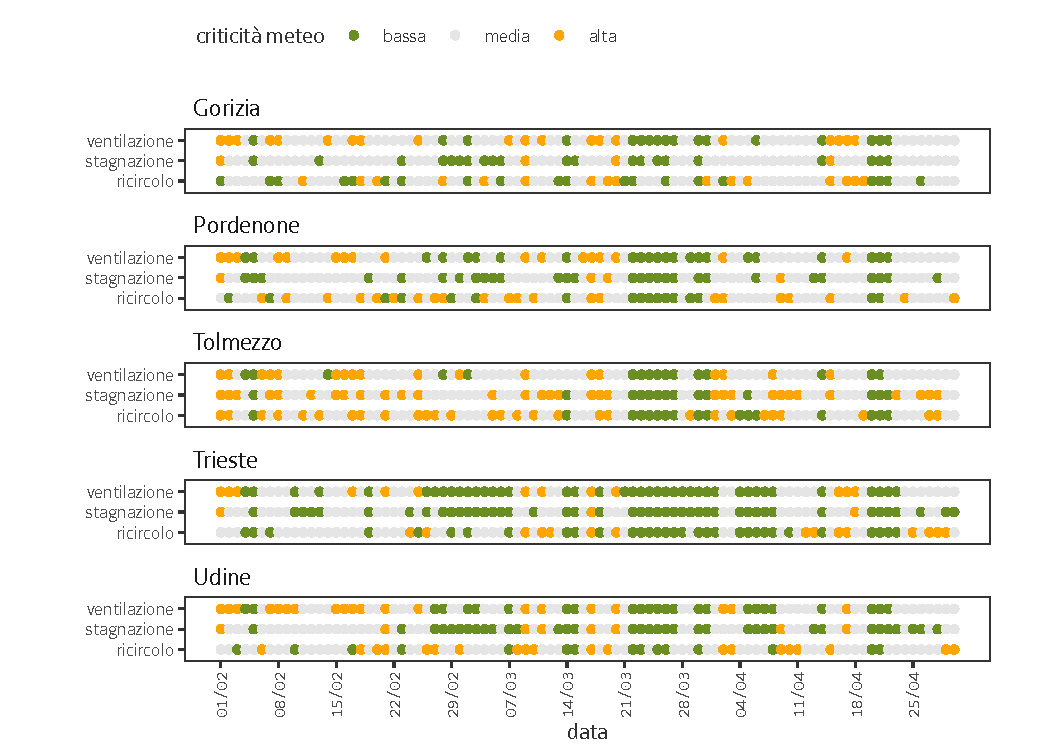
\includegraphics[width=\textwidth]{{figs/RecStaVen_20200201-20200430}.pdf}
    \caption[Indicatori meteo: ricircolo, stagnazione, ventilazione]{Indicatori meteorologici rilevanti per la qualità dell'aria (ricircolo, stagnazione, ventilazione) nel trimestre febbraio-aprile 2020}
    \label{fig:RSV}
\end{figure}

\begin{figure}
    \centering
    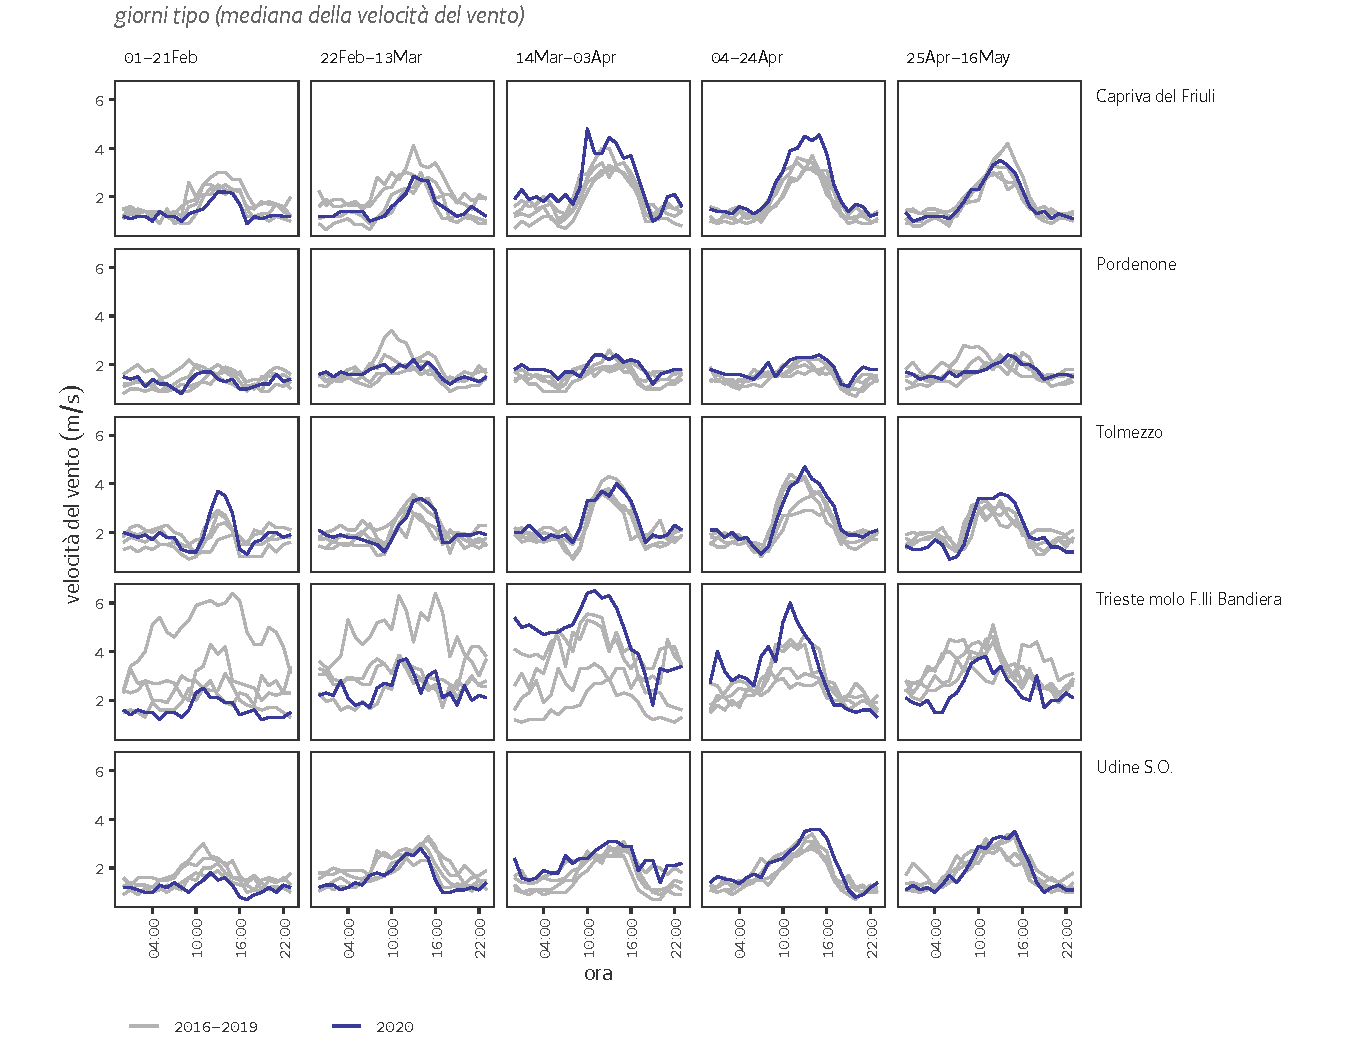
\includegraphics[width=\textwidth]{{figs/WindSpeed_MedianDay_LastVsPast_20200201-20200516}.pdf}
    \caption[Giorni tipo della velocità del vento]{Giorni tipo della velocità del vento, calcolati ogni tre settimane come mediana per ciascuna delle 24 ore. Confronto del 2020 con i 4 anni precedenti.}
    \label{fig:giornivento}
\end{figure}
